\chapter{Supplementary Figures}
\begin{figure}[!ht]
\begin{center}
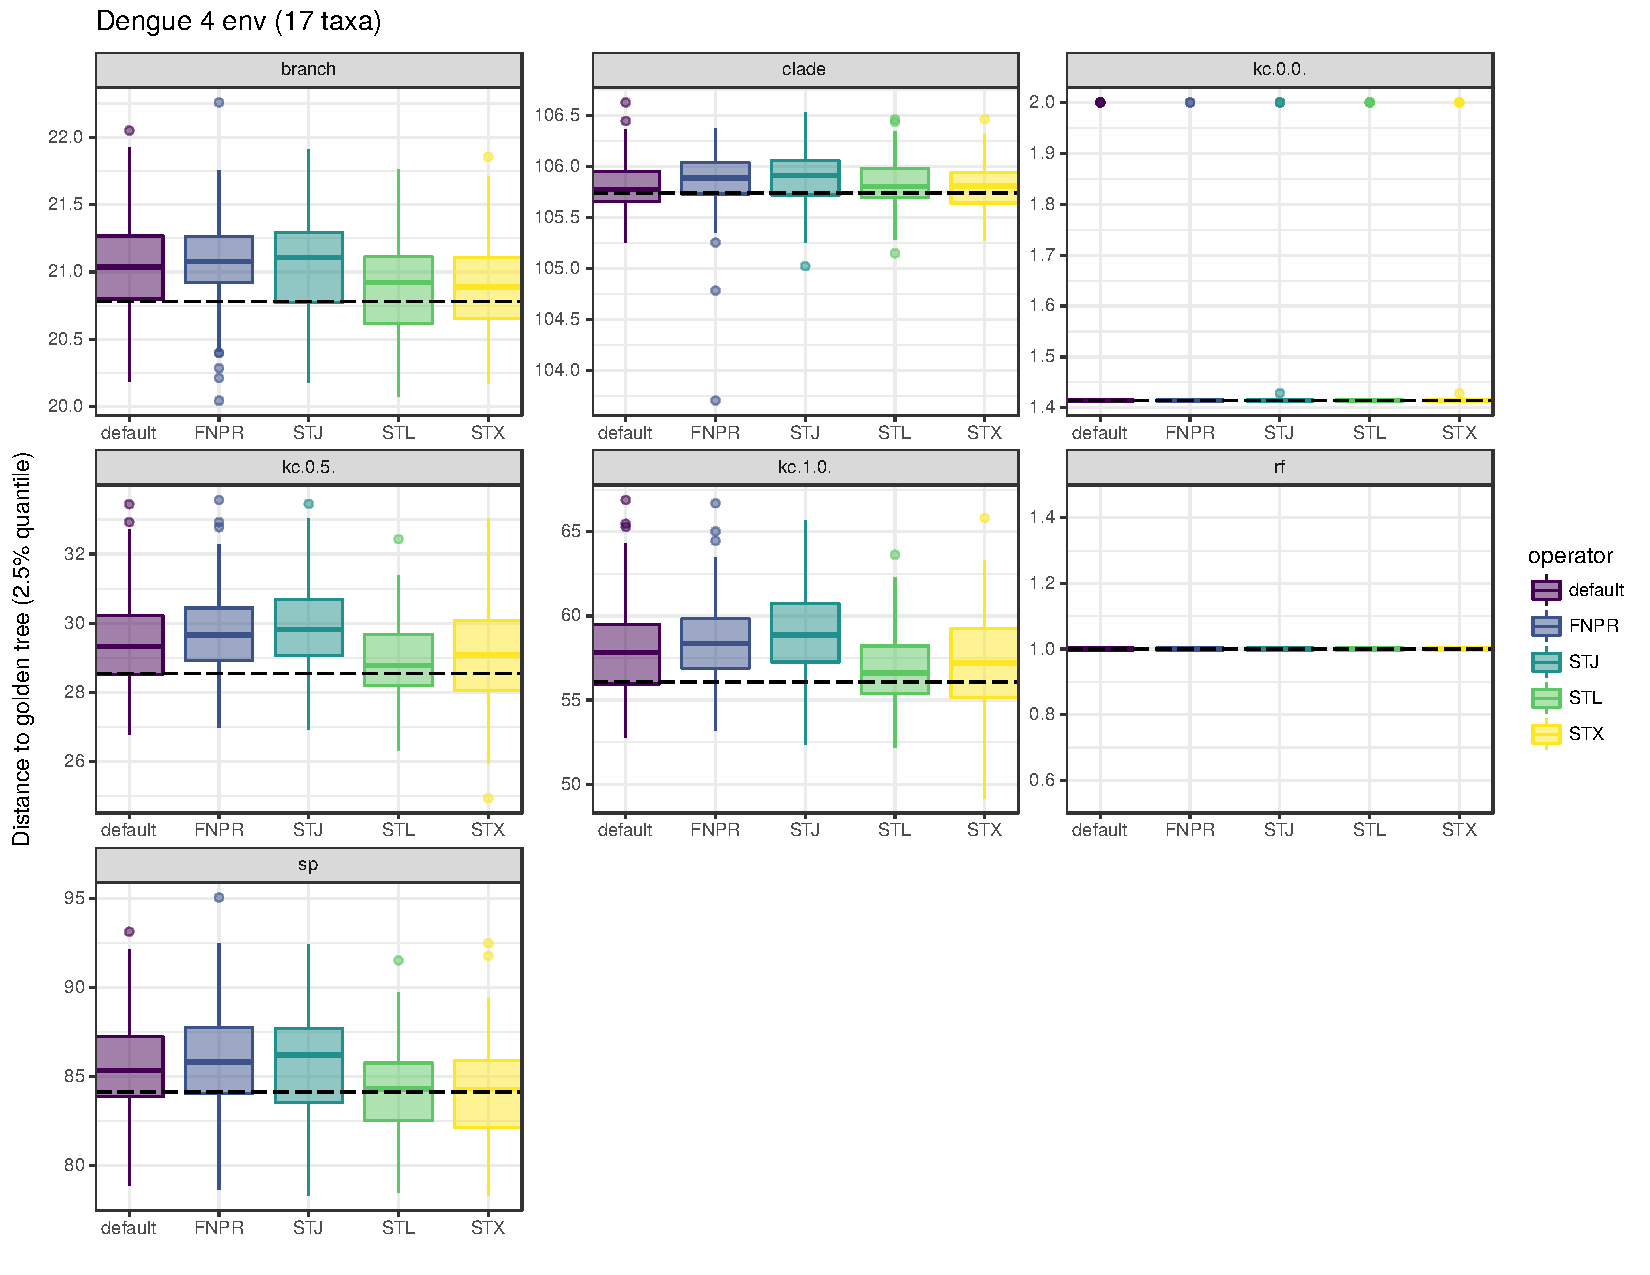
\includegraphics[scale=0.6]{\dir/figs/distance_true_denv4env_lwr.pdf} 
\end{center}
 \caption[Lower quantile (2.5\% quantile) distance to true golden true tree for several combinations of MCMC transition kernels, Dengue 4 \textit{env} data set (17 taxa).]{\textbf{Lower quantile (2.5\% quantile) distance to true golden true tree for several combinations of MCMC transition kernels, Dengue 4 \textit{env} data set (17 taxa).}
  }
  Boxplots show the results of $100$ replicates per data set.
  Vertical tiles show different metrics and the dashed lines show 2.5\% quantiles for the target distributions shown in Figure~\ref{fig:target_golden}.
 \label{sfig:distance_true_denv4_lwr}
\end{figure}

\begin{figure}[!ht]
\begin{center}
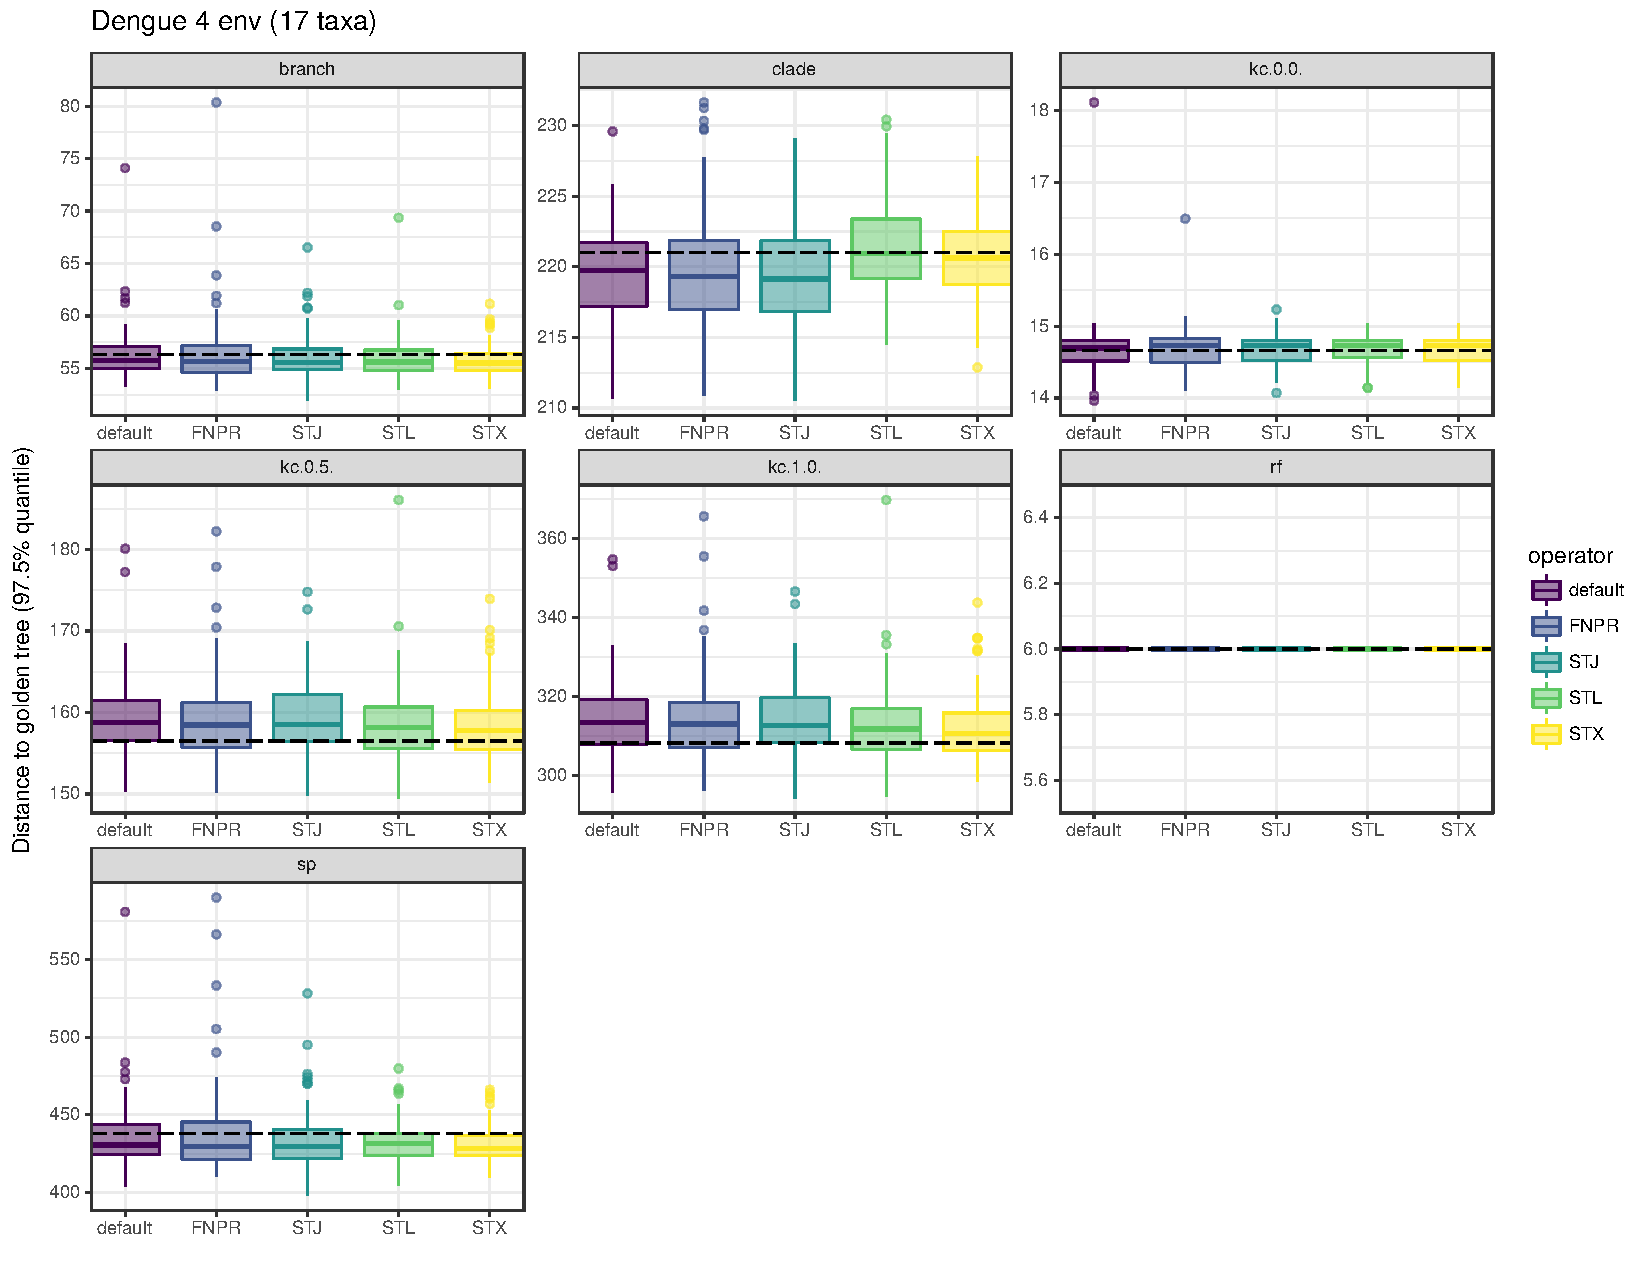
\includegraphics[scale=0.6]{\dir/figs/distance_true_denv4env_upr.pdf} 
\end{center}
 \caption[Upper quantile (97.5\% quantile) distance to true golden true tree for several combinations of MCMC transition kernels, Dengue 4 \textit{env} data set (17 taxa).]{\textbf{Upper quantile (97.5\% quantile) distance to true golden true tree for several combinations of MCMC transition kernels, Dengue 4 \textit{env} data set (17 taxa).}
  }
  Boxplots show the results of $100$ replicates per data set.
  Vertical tiles show different metrics and the dashed lines show the 97.5\% quantiles the target distributions shown in Figure~\ref{fig:target_golden}.
 \label{sfig:distance_true_denv4_upr}
\end{figure}

\begin{figure}[!ht]
\begin{center}
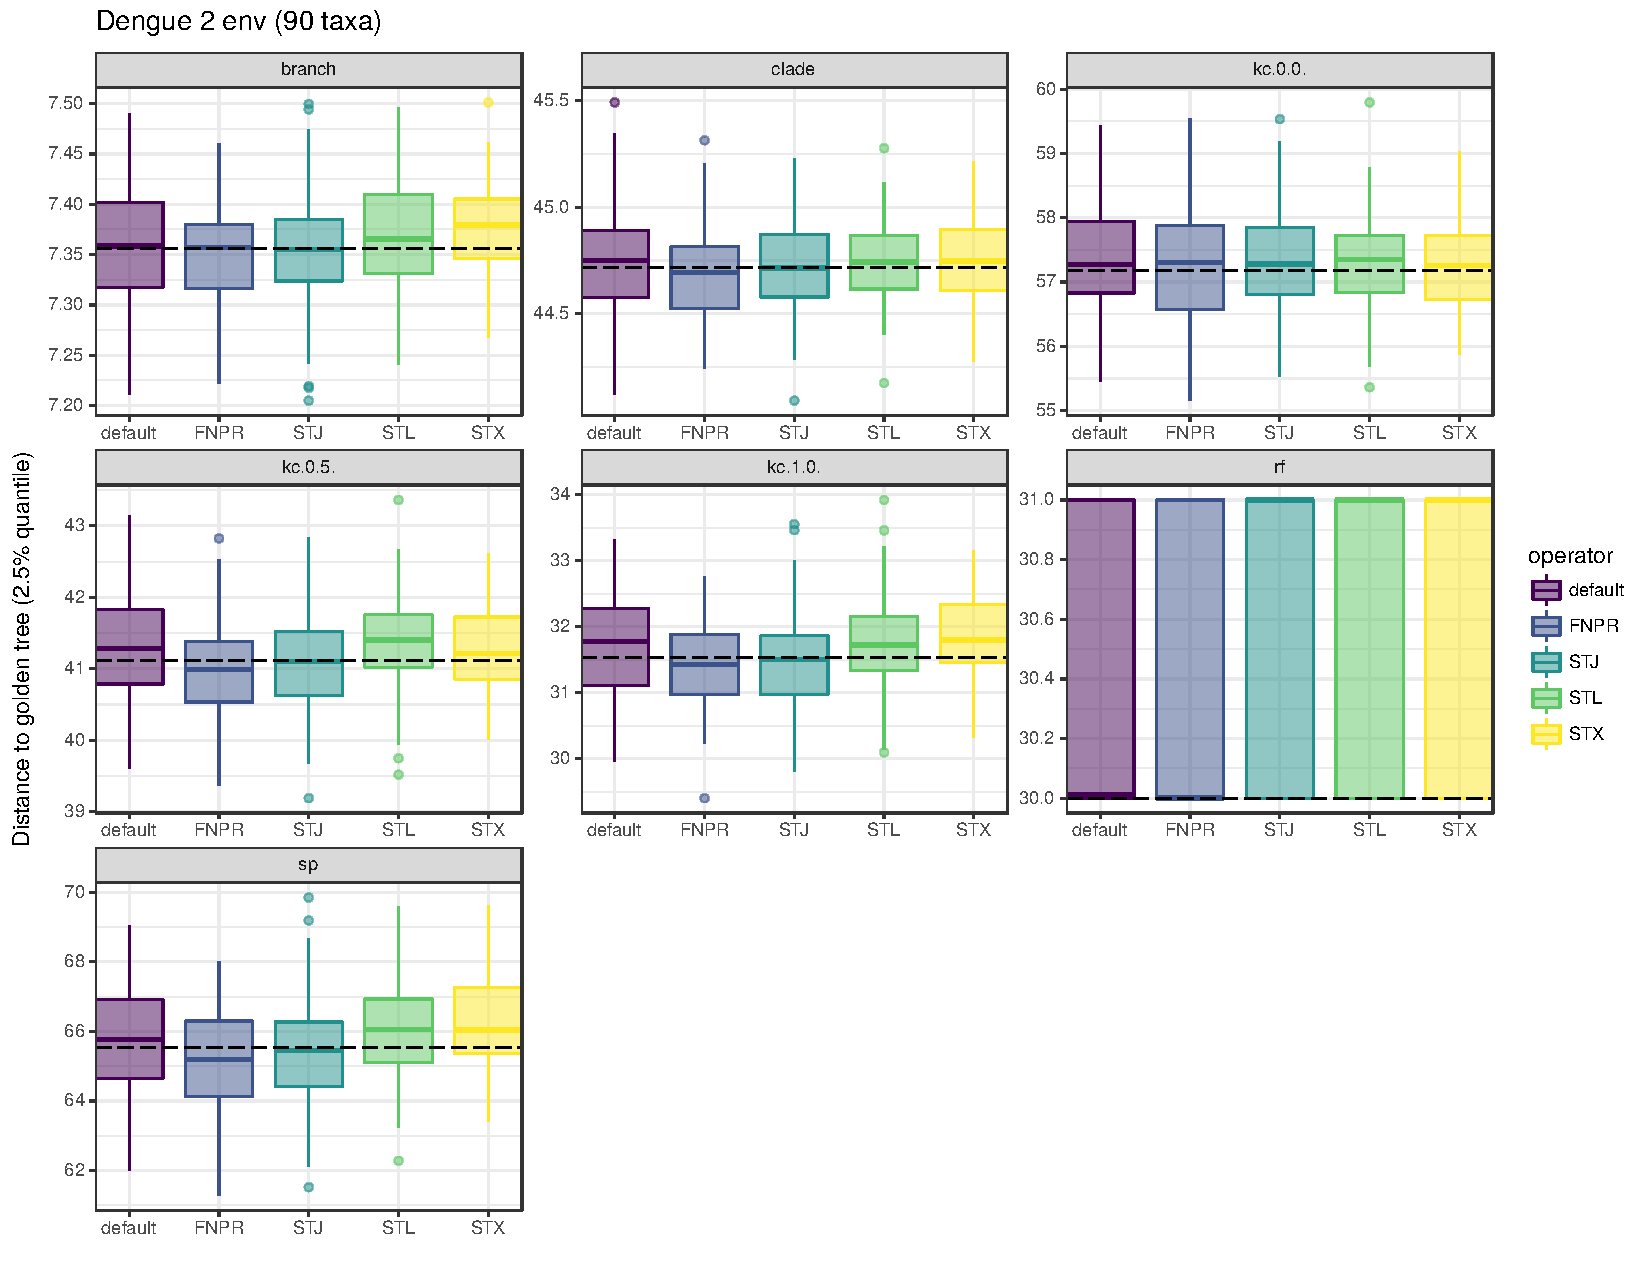
\includegraphics[scale=0.6]{\dir/figs/distance_true_denv2env_lwr.pdf} 
\end{center}
 \caption[Lower quantile (2.5\% quantile) distance to true golden true tree for several combinations of MCMC transition kernels, Dengue 2 \textit{env} data set (90 taxa).]{\textbf{Lower quantile (2.5\% quantile) distance to true golden true tree for several combinations of MCMC transition kernels, Dengue 2 \textit{env} data set (90 taxa).}
  }
  Boxplots show the results of $100$ replicates per data set.
  Vertical tiles show different metrics and the dashed lines show 2.5\% quantiles for the target distributions shown in Figure~\ref{fig:target_golden}.
 \label{sfig:distance_true_denv2_lwr}
\end{figure}

\begin{figure}[!ht]
\begin{center}
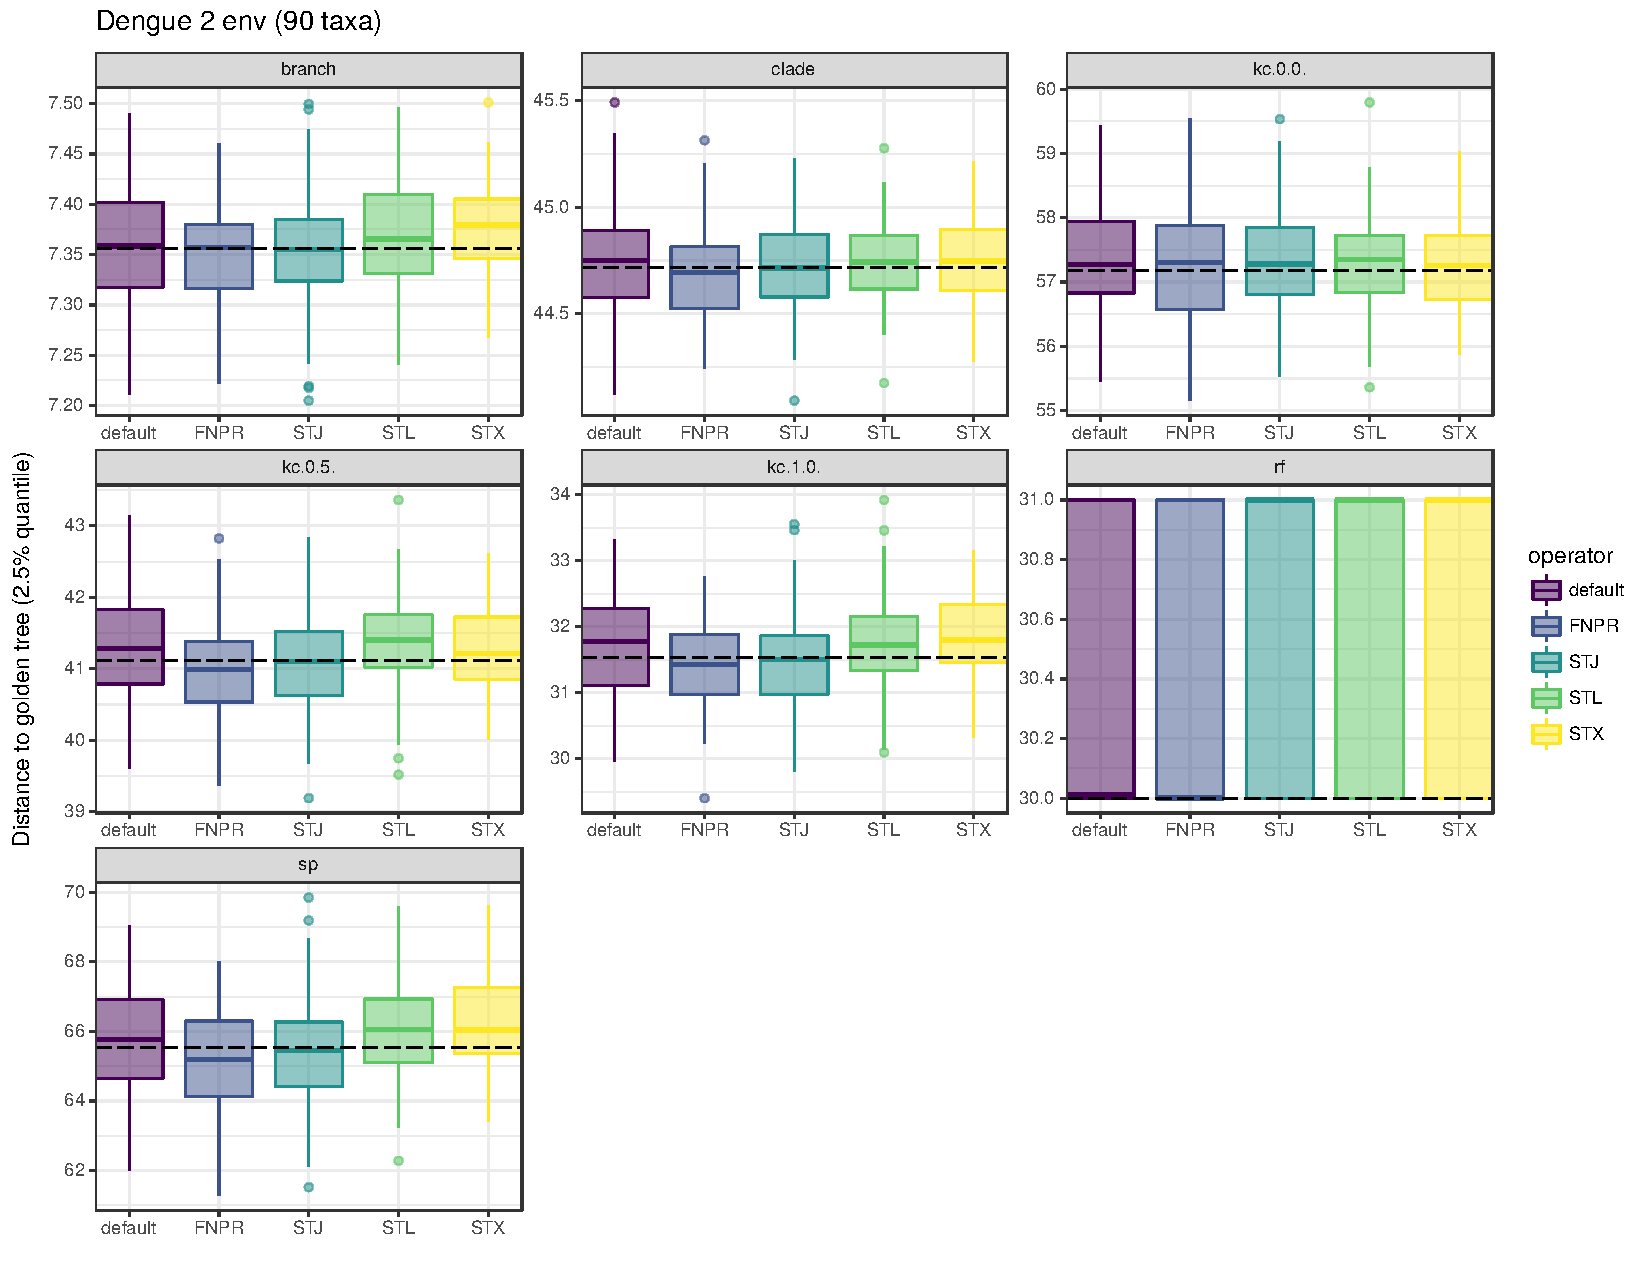
\includegraphics[scale=0.6]{\dir/figs/distance_true_denv2env_lwr.pdf} 
\end{center}
 \caption[Upper quantile (97.5\% quantile) distance to true golden true tree for several combinations of MCMC transition kernels, Dengue 2 \textit{env} data set (90 taxa).]{\textbf{Upper quantile (97.5\% quantile) distance to true golden true tree for several combinations of MCMC transition kernels, Dengue 2 \textit{env} data set (90 taxa).}
  }
  Boxplots show the results of $100$ replicates per data set.
  Vertical tiles show different metrics and the dashed lines show the 97.5\% quantiles the target distributions shown in Figure~\ref{fig:target_golden}.
 \label{sfig:distance_true_denv2_upr}
\end{figure}

\begin{figure}[!ht]
\begin{center}
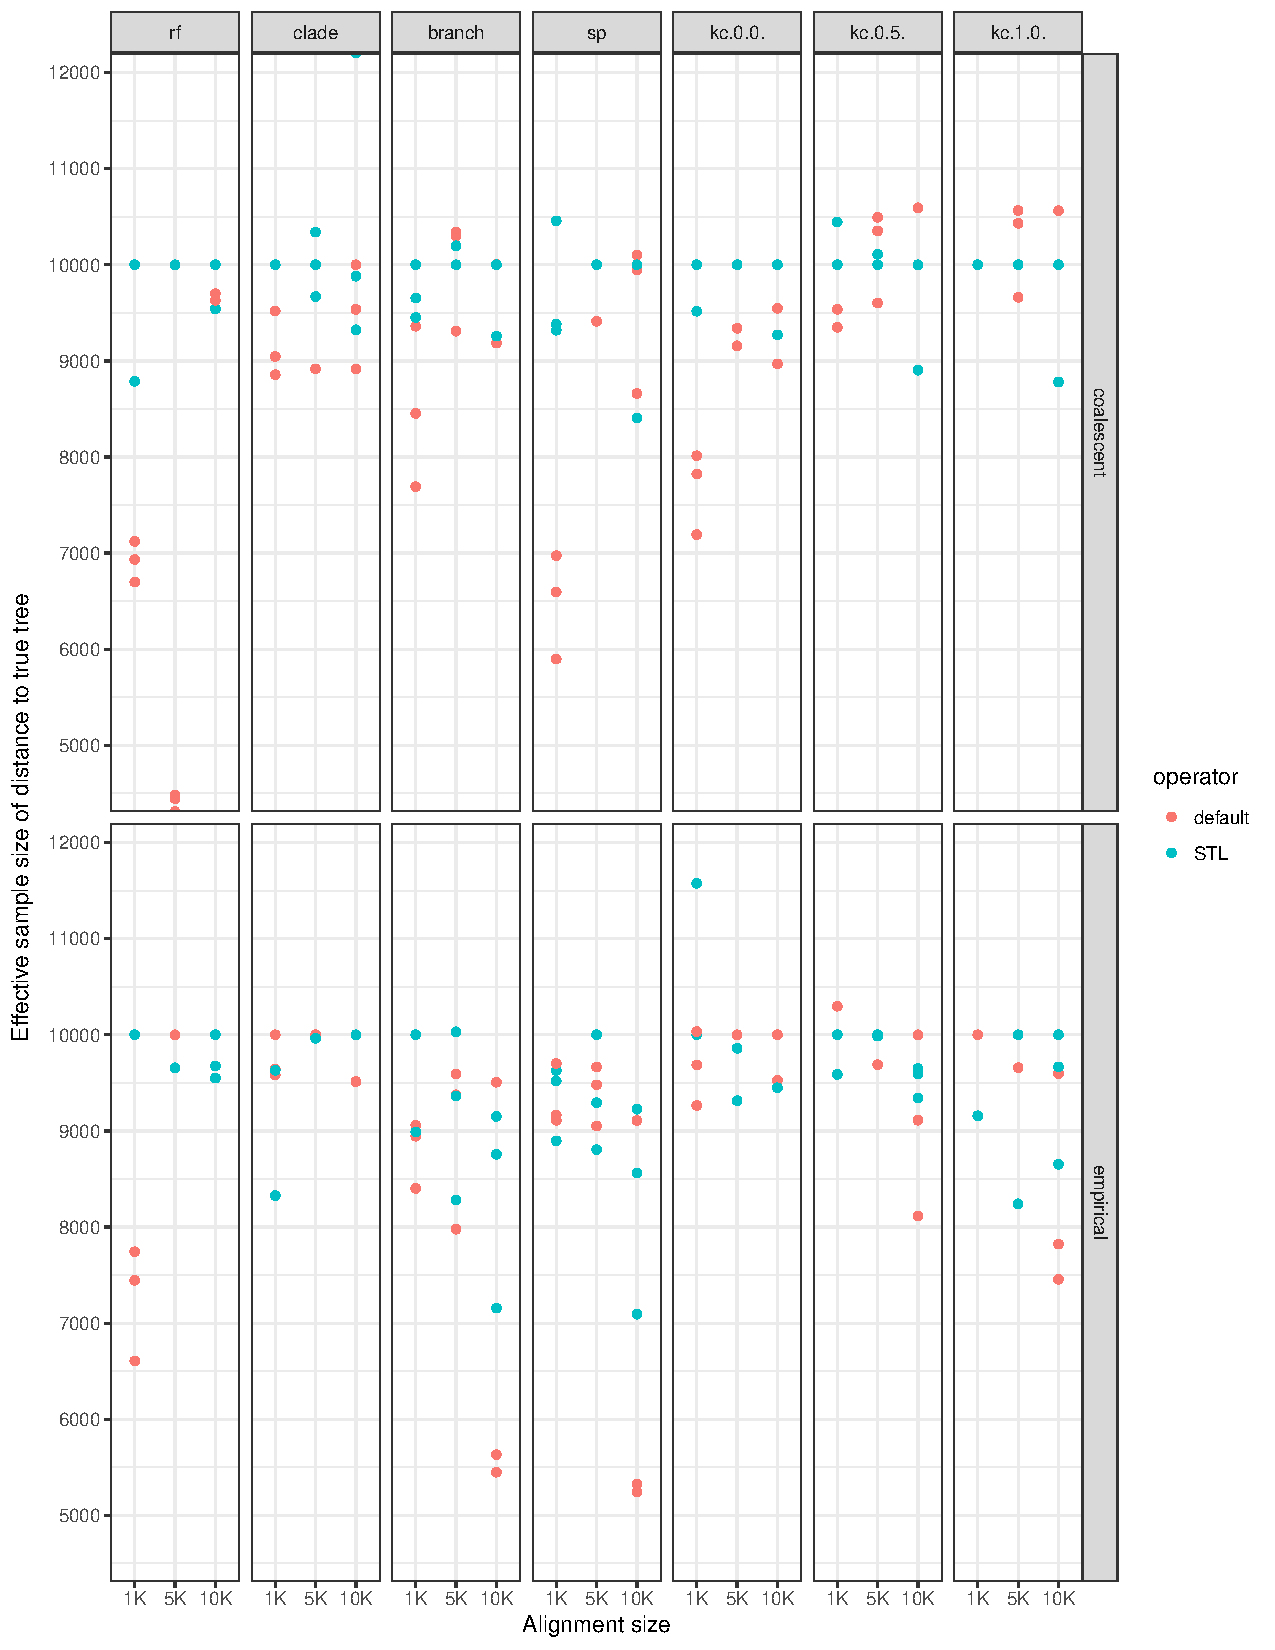
\includegraphics[scale=0.6]{\dir/figs/ESS_distances_50taxa.pdf} 
\end{center}
 \caption[Effective sample sizes of the distance to true tree for different MCMC transition kernels, simulated data sets (50 taxa).]{\textbf{Effective sample sizes of the distance to true tree for different MCMC transition kernels, simulated data sets (50 taxa)}.
  }
  I ran each chain for 10 million iterations, sampling trees every 1000 iterations.
  Each panel shows three replicates per data set.  
  Vertical tiles show different metrics and vertical tiles show the two base trees used to simulate the data (coalescent and empirical).
 \label{sfig:ess_true_50taxa}
\end{figure}